%!TEX root = ../../../super_main.tex

\section{Locked Features for Citizens}
\label{sec:locked_features_for_citizens}

When viewing categories that have been assigned to a citizen profile, it is not possible to change the pictogram of a category, the name of a category, or copy their categories to other citizens, since the categories that are assigned to the citizen are derived categories of one that is located on the institution. This is enforced such that it is possible to propagate changes from the super-category to the child-categories, which for example could be changing the name of a category across all users that have the category.\\

When locking features for citizens it has been decided that we use the \androidinline{View.setEnabled()} method on \androidinline{GirafButtons} with the value \androidinline{false}, which will automatically gray out the button, instead of hiding the button. We then set a special click-listener on the button that is only active while the button is not enabled. This allows users of the \ct to press buttons that are disabled and then give us the possibility of telling the user the correct way of using the button. This has been implemented on two \androidinline{GirafButtons} in the \ct, namely the settings button and the copy-category button, since these are not available to citizen categories. Examples of enabled and clickable buttons can be seen in \figref{fig:ct_enabled_buttons}, while an example of disabled clickable buttons can be seen in \figref{fig:ct_disabled_buttons}. The dialog which is shown when you click one of the disabled buttons can be seen in \figref{fig:notifydialog_on_locked_click}. This dialog contains the text \translated{Det er ikke muligt at lave indstillinger for bruger-kategorier. Vend i stedet tilbage til hovedoversigten}{It is not possible to adjust settings for user-categories. Return to the main view instead.}. This text can be changed if the disable functionality is used somewhere else. 

\begin{figure}[!htbp]
        \centering
        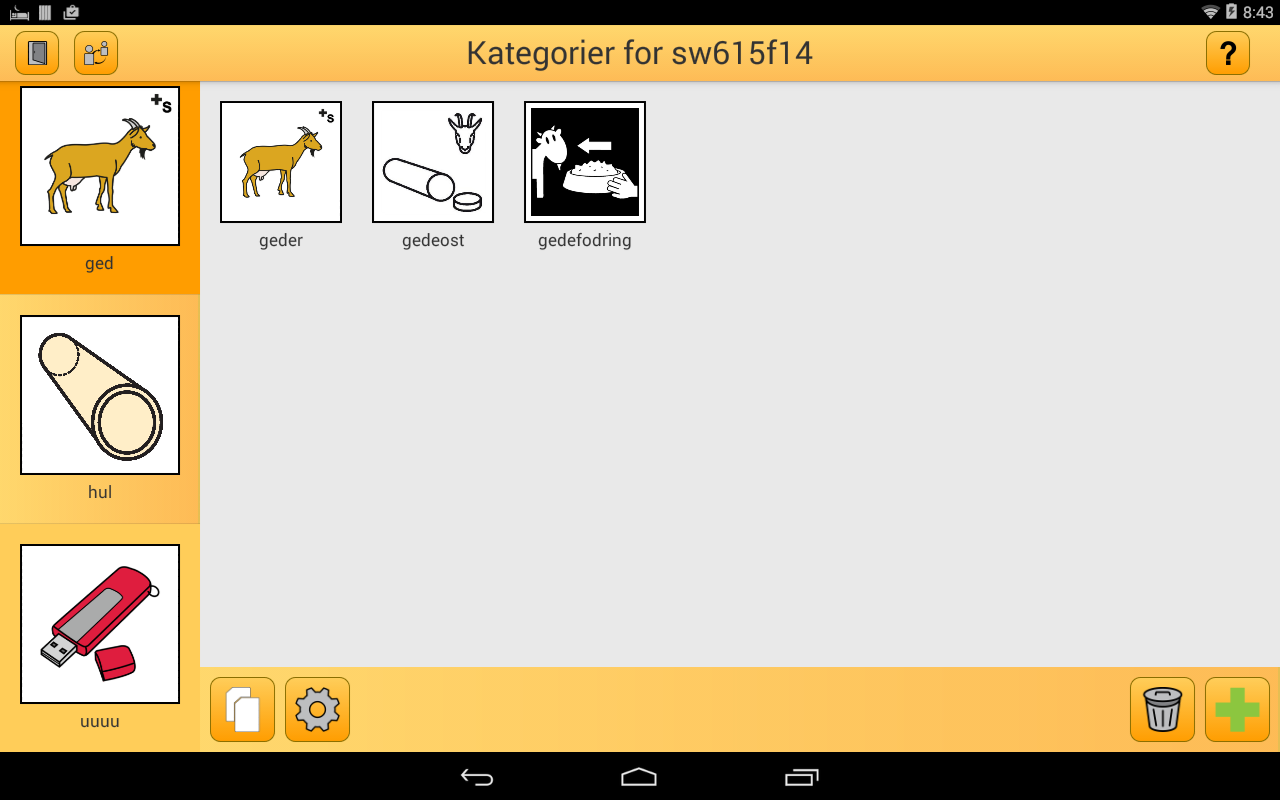
\includegraphics[width=0.75\textwidth]{sprint_three/locked_features_for_citizens/buttons_for_institution}
        \caption{\ct enabled buttons}
        \label{fig:ct_enabled_buttons}
\end{figure}

\begin{figure}[!htbp]
        \centering
        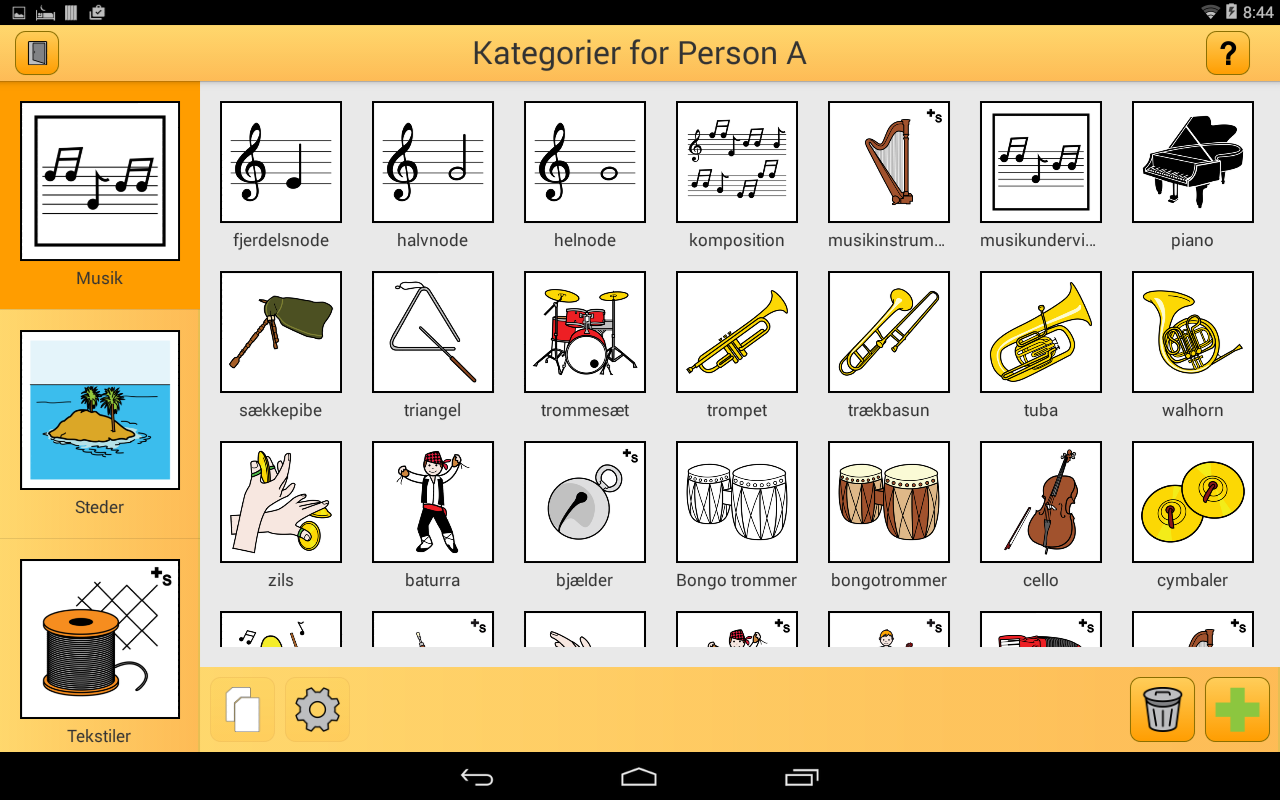
\includegraphics[width=0.75\textwidth]{sprint_three/locked_features_for_citizens/buttons_for_citizen}
        \caption{\ct disabled buttons}
        \label{fig:ct_disabled_buttons}
\end{figure}

\begin{figure}[!htbp]
        \centering
        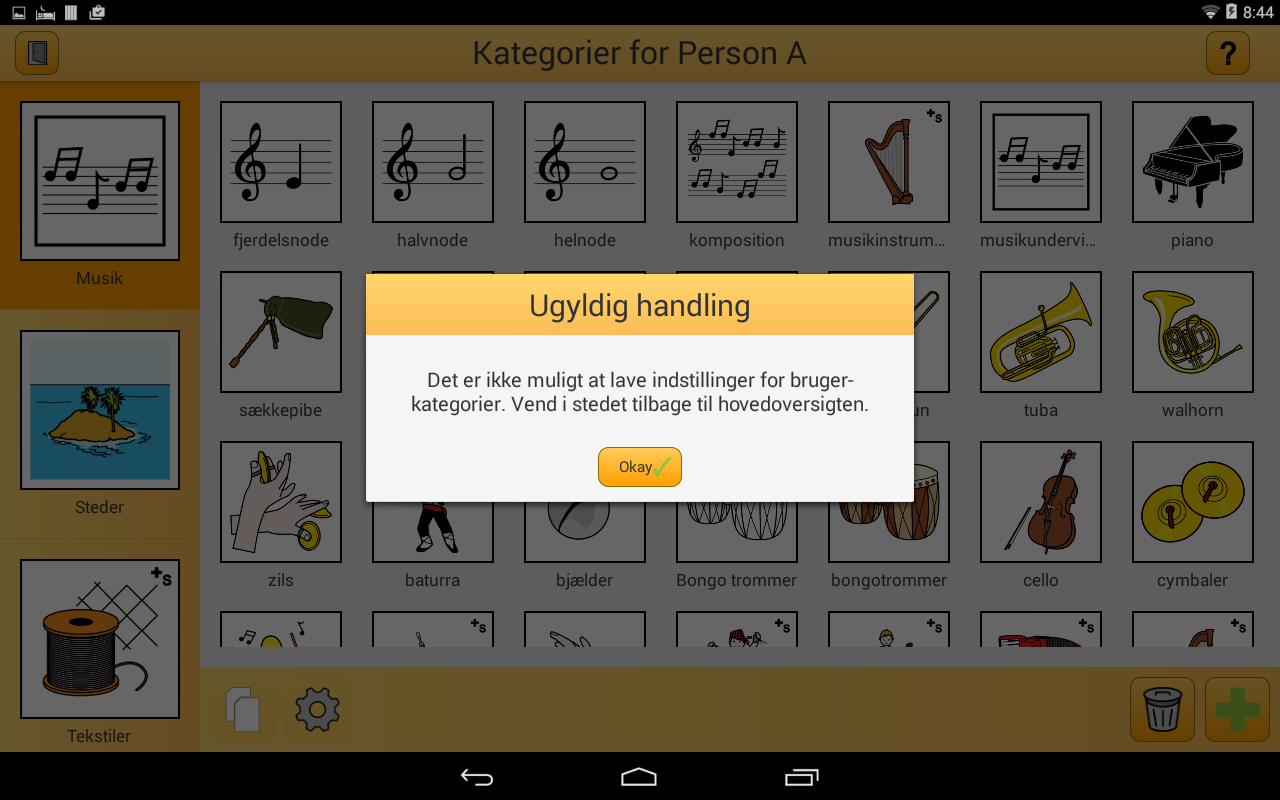
\includegraphics[width=0.75\textwidth]{sprint_three/locked_features_for_citizens/notifydialog_on_locked_click}
        \caption{Dialog shown when clicking disabled button}
        \label{fig:notifydialog_on_locked_click}
\end{figure}